\section{Metodología}
En esta sección presenta una propuesta para evaluar la precisión de modelos de regresión lineal mediante intervalos de confianza para el coeficiente de determinación \(R^2\). Se consideran modelos Exactos-Precisos (EP) y Exactos-Imprecisos (EI) bajo diferentes supuestos: Normalidad-Varianza Constante (NVC), No Normalidad-Varianza Constante (NNVC), Normalidad-Varianza Distinta (NVD) y No Normalidad-Varianza Distinta (NNVD). Se aplican esquemas de Bootstrap, incluyendo algoritmos de \textcite{wu-1986}, \textcite{liu-1988}, \textcite{zacarias-2023} y \textcite{balam-2012}, utilizando distintas técnicas de remuestreo y estimadores robustos según el cumplimiento de supuestos.

La metodología se valida mediante la simulación de 24,000 modelos distribuidos en 48 escenarios, cada uno con 500 modelos y 5 réplicas. Se consideran factores como el tamaño de muestra, precisión y supuestos. Se construyen intervalos Bootstrap (percentil y BCa) para determinar la precisión de \(R^2\), evaluando su eficacia mediante la frecuencia con la que los intervalos contienen el valor verdadero y analizando su ancho. Se realiza un análisis ANOVA factorial para identificar diferencias significativas entre los intervalos, complementado con pruebas de Tukey. Las simulaciones y análisis se implementan en el lenguaje R.


\subsection{Una Propuesta para Evaluar la Precisión de un Modelo}

Desarrollar la metodología para medir la precisión de un modelo con la técnica de regresión lineal por medio de intervalos de confianza basado en diferentes esquemas de remuestreo Bootstrap. 
\begin{figure}
	\centering 
	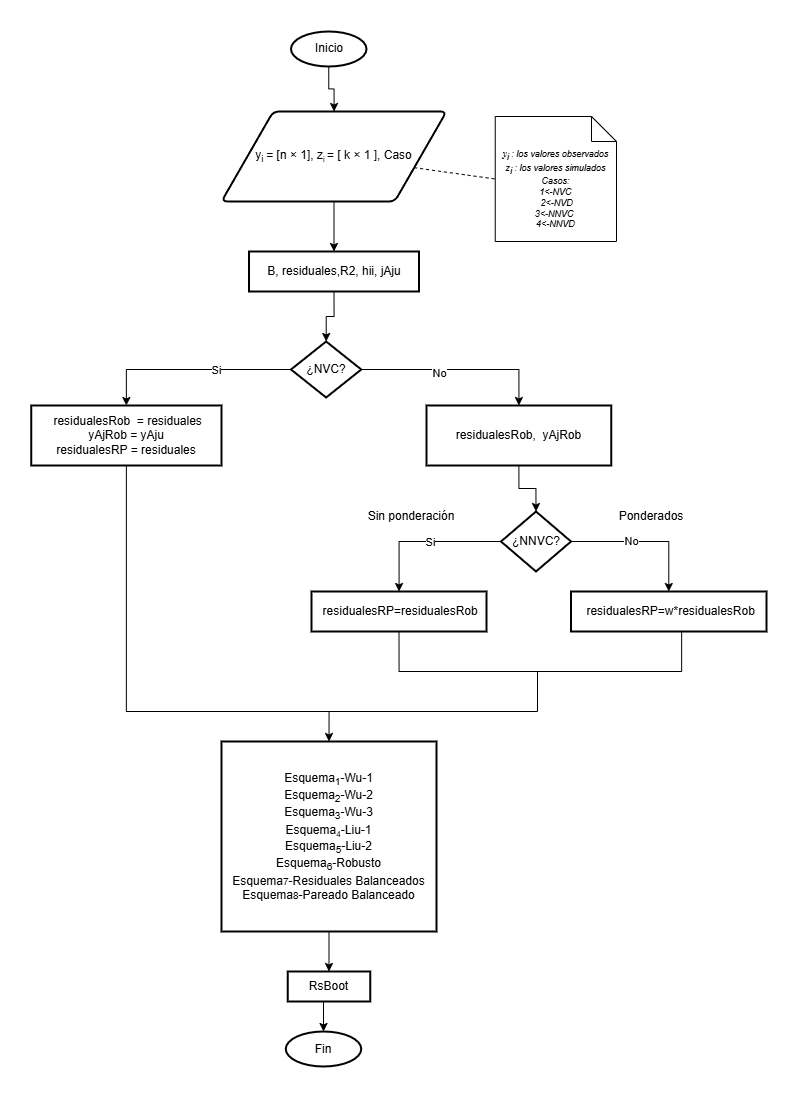
\includegraphics[width=0.70\linewidth]{img/metodo.png} 
	\caption{Algoritmo para los diferentes esquemas Bootstrap.}
\end{figure}
\

































\vspace{1.5cm}
\subsection{Precisión de modelos que cumplen el supuesto de normalidad y varianza constante}
Determinar la precisión de un modelo cuando se cumplan los supuestos de normalidad y varianza constante.
\vspace{1.5cm}





\subsection{Precisión de modelos que no cumplen el supuesto de normalidad y/o varianza constante}
Determinar la precisión de un modelo cuando no se cumplan los supuestos de normalidad y/o varianza constante.
\vspace{1.5cm}
	 
	 
\subsection{Estudio de simulación para la evaluación de la propuesta}
\vspace{1.5cm}

\subsubsection{Simulación de modelo}
Simular modelos exactos-precisos (EP) y modelos exactos-imprecisos (EI) mediante la propuesta de Febles (2014) y Zacarías (2023); cuando se cumplan o no los supuestos de normalidad e igualdad de varianzas.

%aqui va el diagrama
Diseñar e implementar un estudio de simulación para evaluar la eficacia de la metodología propuesta.
	 \vspace{1.5cm}
	 	 
	 	 
	 	 
	 	 
\subsection{Análisis estadísticos}
Para cada supuesto (NVC, NNVC, NVD, NNVD) se utilizó ANOVA en un arreglo factorial de tres factores seguido de la comparación múltiple de Tukey (Montgomery, 2017), para determinar el comportamiento de la eficacia de dos ICB en la evaluación de la precisión, bajo ocho esquemas de remuestreo, seis tamaños de muestra y dos tipos de modelo. Cabe señalar que, en cuatro de los ocho análisis de varianza realizados se eliminaron valores atípicos para el logro del cumplimiento de los supuestos del ANOVA.
Las pruebas estadísticas se consideraron significativas cuando  y se utilizó el paquete estadístico STATGRAPHICS Centurion 19 (Statgraphics, 2024).




